\documentclass{beamer}
\usetheme{AnnArbor}
\usecolortheme{crane}
\usepackage[utf8]{inputenc}
\usepackage{graphicx}
\title{5 Things I Learnt from My First Himalayan Trek}
\subtitle{"Where the Strange Trails Go Down"}
\author{Sankalp Shekhar}
\date{\today}
\institute{MIT, Manipal}
\date{\today}
\begin{document}
\frame{\titlepage}
\begin{frame}
\frametitle{Table of Contents}
\tableofcontents[]
\end{frame}
\section{Introduction}
\begin{frame}
\frametitle{Introduction}
 \textit{"In every walk in with nature, one receives far more than he seeks." -John Muir}
 	\begin{figure}[h] 
 		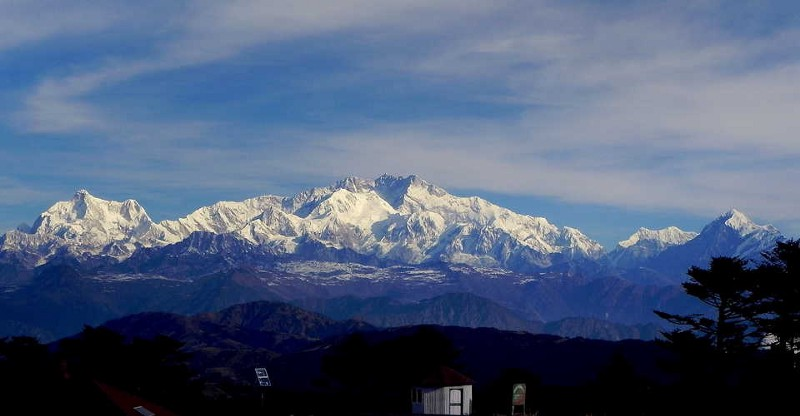
\includegraphics[width=\linewidth]{latex2.jpeg}
 		\caption{The Kanchenjunga, as seen from Sandakphu. Image Courtesy:Souvo Chowdhury}
 		\label{figref1}
 	\end{figure}
\end{frame}
\tableofcontents
\section{first thing}
\begin{frame}
\frametitle{Trekking is good for health.}
\end{frame}

\end{document}